% ==============
% Main file. Project report on COJAC. It includes all other files.
% ==============

\documentclass[french,11pt]{report}

%% PACKAGES %%
% For Bibliography
\usepackage[square, numbers]{natbib}
% For french support
\usepackage[utf8]{inputenc}
\usepackage[T1]{fontenc}
\usepackage{babel}
% Geometry of document
\usepackage{geometry}
% To include images
\usepackage{graphicx}
% For not floating images
\usepackage[hypcap=false]{caption}
% For links (and table of contents)
\usepackage{hyperref}
% For table
\usepackage{tabularx}
% For text color
\usepackage{xcolor}
% For code syntax highlighter
\usepackage{minted}
% For code background and border
\usepackage{tcolorbox}
\usepackage{etoolbox}
% Prevent the ~ to be written in superscript in minted environment
\usepackage[T1]{fontenc}
\usepackage{lmodern}
% For Landscape
\usepackage{pdflscape}
% For appendices
\usepackage[toc,page]{appendix}
% For glossaries
\usepackage[nopostdot,section=chapter,numberedsection]{glossaries}
\usepackage{caption}
\usepackage{subcaption}


%% COMANDS %%
% print todo and the text in red and show an error
\newcommand{\todo}[1]{
    \textcolor{red}{\textbf{TODO: #1}}
    \PackageError{Document}{TODO}{#1!}
}
% display the inline code with a background and a border
\newcommand{\inputmintedcolor}[3][firstline=1]{\begin{tcolorbox}\inputminted[breaklines,xleftmargin=20pt,linenos,#1]{#2}{#3}\end{tcolorbox}}
% get the type of a section and its number where a label has been defined
\newcommand*{\fullref}[1]{\hyperref[{#1}]{\autoref*{#1} \nameref*{#1}}}
% format a title to use in subsection
\newcommand{\subtitle}[1]{\vspace{5mm}{\large\textsc{\textbf{#1}}} \par}
% Rename chapter for appendices
\renewcommand{\appendixpagename}{Annexes}
\renewcommand{\appendixtocname}{Annexes}


%% ENVIRONNMENT %%
\newlength{\currentparskip}
\newenvironment{minipage2} % keep the same space between paragraphs
    {\setlength{\currentparskip}{\parskip} % save the parskip
    \begin{minipage}{\linewidth}
    % parskip is reset to 0 inside a minipage environment
    \setlength{\parskip}{\currentparskip} % restore the parskip
    }
    {\end{minipage}}


%% CONFIG %%
% Default image directory
\graphicspath{{images/}}

% Set minted background and border
% It is in another file, because it will probably break the LaTeX syntax highlighting

% Add box around code
\BeforeBeginEnvironment{minted}{\begin{tcolorbox}}%
\AfterEndEnvironment{minted}{\end{tcolorbox}}%

\setlength{\parindent}{0em}
\setlength{\parskip}{1em}

\newgeometry{left=3cm, right=3cm, top=3cm, bottom=3cm}

\bibliographystyle{plainnat}

% Avoid page breaks before lists
\makeatletter
\@beginparpenalty=10000
\makeatother

% Avoid widow and orphan lines
\widowpenalty10000
\clubpenalty10000


%% DOCUMENT INFO %%
% PROJECT CONFIGURATION
\def\projectname{Intégration des nombres complexes et des Unum en Java avec COJAC}
\def\projectinfo{Travail de bachelor}

% DOCUMENT CONFIGURATION
\def\department{Filière Informatique 2020-2021}
\def\student{Cédric Tâche}
\def\professor{Frédéric Bapst}
\def\expert{Baptiste Wicht}
\def\classe{Classe I3}

\title{Rapport}
\author{Cédric Tâche}
\def\version{0.1}


%% GLOSSARY %%
% ==============
% Create the glossary
% ==============

\makeglossaries

\newglossaryentry{JDK}
{
    name = {Java Development Kit (JDK)},
    text = {JDK},
    description = {Un ensemble d'outils utilisés pour développer une application Java. Cela inclus la JVM, le compilateur, etc.}
}

\newglossaryentry{JVM}
{
    name = {Java virtual machine (JVM)},
    text = {JVM},
    description = {Une machine virtuelle qui permet d'exécuter des programmes écrits en Java ainsi qu'avec certains autres langages. Les programmes exécutés doivent préalablement être compilés en Bytecode.}
}

\newglossaryentry{Unums}
{
    name = {Universal number (Unum)},
    text = {Unum},
    description = {Un nouveau format de stockage pour les nombres réels dont le but est de remplacer les nombres à virgule flottante.}
}

\newglossaryentry{JNI}
{
    name = {Java Native Interface (JNI)},
    text = {JNI},
    description = {JNI permet d'appeler des fonctions natives (généralement écrites en C) depuis un programme Java.}
}

\newglossaryentry{COJAC}
{
    name = {COJAC},
    description = {Un outil capable de modifier le comportement d'une application Java à l'aide d'un agent Java.}
}

\newglossaryentry{Maven}
{
    name = {Maven},
    description = {Un outil d'automatisation pour gérer les dépendances et compiler une application.}
}

\newglossaryentry{Java-agent}
{
    name = {agent Java},
    plural = {agents Java},
    description = {Un objet Java qui peut intercepter le chargement d'une classe et modifier son Bytecode.}
}

\newglossaryentry{Bytecode}
{
    name = {Bytecode},
    description = {Le langage utilisée par la JVM}
}

\newglossaryentry{Behaviour}
{
    name = {Behaviour},
    description = {Un mécanisme de COJAC permettant de modifier les opérations agissant sur les types primitifs.}
}

\newglossaryentry{Wrapper}
{
    name = {Wrapper},
    description = {Un mécanisme de COJAC permettant de remplacer les \textit{floats} et \textit{doubles} par un objet.}
}

\newglossaryentry{Complex-number}
{
    name = {nombre complexe},
    plural = {nombres complexes},
    description = {Une extension des nombres réels permettant de faire certaines opérations mathématiques impossibles avec les nombres réels.}
}

\newglossaryentry{Posit}
{
    name = {Posit},
    description = {Un nouveau format de stockage spécifié dans les Unums III.}
}

\newglossaryentry{SoftPosit}
{
    name = {SoftPosit},
    text = {\textit{SoftPosit}},
    description = {Une librairie C permettant de réaliser certains calculs avec des Unums.}
}

\newglossaryentry{JAR}
{
    name = {Java ARchive (JAR)},
    text = {JAR},
    description = {Un fichier regroupant toutes les ressources et toutes les classes utilisées par une application Java.}
}

\newglossaryentry{Makefile}
{
    name = {Makefile},
    text = {\textit{Makefile}},
    description = {Un fichier de configuration composé de règles permettant de compiler un programme.}
}


\begin{document}


%% TITLE %%
\pagenumbering{alph}
\makeatletter
\begin{titlepage}

    \centering

    
\includegraphics{title/Logo_HEIA-FR.png}

    \LARGE{
        \textit{\department}
        \vspace*{0.8 cm}

        \projectname
        \vspace*{0.5 cm}

        {\small }

        \classe
        \vspace*{0.5 cm}

    	\rule{\linewidth}{0.2 mm} \\[0.5 cm]
    	\@title

    	\rule{\linewidth}{0.2 mm} \\[0.5 cm]
	}
	\Large{
    	\projectinfo \\[2.0 cm]

    	Version: \version \\[3.0 cm]

    	\begin{tabular}{l@{\hspace{1cm}}l}
    		Student : & \student \\[2ex]
    		Professor : & \professor \\[2ex]
    		Expert : & \expert \\[2ex]
    	\end{tabular}
	}

\end{titlepage}
\makeatother


%% TABLE OF VERSIONS %%
\pagenumbering{Roman}
\section *{Table des versions}
\vspace*{0.5 cm}

\begin{table}[h]
    \begin{tabularx}{\columnwidth}{ | p{3.5em} |p{7em} | p{6.5em} | X |}
        \hline
        \textbf{Version} & \textbf{Date} & \textbf{Author} & \textbf{Description} \\
        \hline
        0.1 & 03.06.2021 & Cédric Tâche & Création de la structure \\
        0.2 & 07.06.2021 & Cédric Tâche & Description de Maven et du problème de compilation \\
        \hline
    \end{tabularx}
\end{table}

\newpage


%% TABLE OF CONTENTS %%
\hypersetup{
	hidelinks,
	allcolors=black,
	linktocpage,
	linktoc=all
}
\tableofcontents
\newpage


%% CONTENT %%
\pagenumbering{arabic}

% ==============
% This is the main content, it includes all chapters and appendices
% ==============

\chapter{Introduction}

La plupart des langages de programmation offrent des capacités similaires pour stocker des nombres et effectuer des calculs. Ces langages permettent, entre autres, d'utiliser  des nombres réels.

Ces nombres réels ont tout de même des limitations. Ils sont limités au domaine du réel. De plus, les nombres à virgule flottante sont souvent inexacts. Par conséquent, lorsque les erreurs s'accumulent, le résultat d'un calcul peut être très éloigné de la réponse exacte.

Pourtant, d'autres alternatives existent. Les nombres complexes sont couramment utilisés en mathématique et en physique. Ils peuvent être utilisés pour simplifier des réponses utilisant des racines de nombres négatifs ou pour combiner deux quantités réelles telles que la tension et l'intensité en électricité. Quant à eux, les nombres réels peuvent aussi être représentés différemment. Les \textbf{universal numbers} (\textbf{unums}) sont une représentation alternative possible dont la dernière version est expliquée dans l'article \textit{Beating Floating Point at its Own Game: Posit Arithmetic} \cite{posit}.


\section{Contexte}

En Java, aucun type ni aucune classe dans le JDK permet de gérer des nombres complexes ou des unum, mais il est possible de l'implémenter soi-même. Des librairies pouvant gérer ces éléments peuvent déjà exister.

La première solution pour ajouter ces fonctionnalités et de créer de nouvelles classes: une classe pour les nombres complexes et une classe pour les unums. Ensuite, il faut écrire le code en utilisant directement ces classes. Pour changer le type de calculs effectué (ex: nombre complexe $\rightarrow$ nombre réel), il faut changer le code source de l'application.

COJAC \cite{COJAC} est une librairie Java permettant de modifier les capacités arithmétiques d'un programme Java sans en modifier le code. Elle utilise l'API d'instrumentation et peut transformer les classes et méthodes au runtime pour changer le type de calcul effectué. Ainsi, pour changer le type de calculs effectué (ex: nombre réel $\rightarrow$ nombre complexe), il faut seulement changer l'argument donné à COJAC \cite{COJAC} lors du démarrage de l'application. Ceci ne demande aucune modification dans l'application de l'utilisateur.

\section{Objectifs}

Le but de ce projet est d'ajouter deux nouvelles fonctionnalités à COJAC \cite{COJAC}. COJAC devra permettre de remplacer automatiquement les nombres à virgules flottantes par deux nouveaux types numériques.

\subsection{Intégration des nombres complexes}

Une option de COJAC permettra de changer le comportement des calculs dans l'application de l'utilisateur. Les nombres à virgules flottantes (\textit{float} et \textit{double}) seront remplacés, au runtime, par des nombres complexes. Les opérations arithmétiques telles que l'addition, la soustration, etc. devront être adaptées. De plus, les méthodes souvent utilisées de la librairie standard devront également pouvoir fonctionner. Par exemple, la méthode \textit{Math.sqrt} devra permettre de retourner la racine carrée d'un nombre négatif.

Voici un exemple sans les nombres complexes:
\begin{minted}{Java}
double val = Math.sqrt(-1); // = NaN
val = val * val; // = NaN;
\end{minted}

Avec les nombres complexes, on obtient le résultat suivant:
\begin{minted}{Java}
double val = Math.sqrt(-1); // = i
val = val * val; // = -1;
\end{minted}

\subsection{Intégration des unums}

Une option de COJAC permettra de changer le format de stockage et de calculs des nombres réels. Les unums seront utilisés à la place de la virgule flottante. Par conséquent, les opérations arithmétiques devront être redéfinies pour fonctionner avec ce nouveau format de stockage. Il faudra probablement utiliser JNI pour accéder à une librairie C/C++ permettant d'utiliser les unums, mais d'autres approches restent possibles.

\subsection{Démonstration des deux fonctionnalités}

Des programmes de démonstrations seront réalisés pour montrer ces deux fonctionnalités. Ces démonstrations doivent montrer l'utilité et les avantages de cette approche.

\begin{minipage2}
\section{Objectifs secondaires}

D'autres ajouts de fonctionnalités ou modifications permettraient d'améliorer ce projet.

\subsection{Mise à jour des librairies}

COJAC \cite{COJAC} utilise plusieurs librairies dont les versions sont désormais obsolètes. Il vaut mieux mettre à jour les versions avant de rencontrer des problèmes à cause de versions trop anciennes. Cependant, COJAC \cite{COJAC} devra garantir une compatibilité pour Java 8+.
\end{minipage2}

\subsection{Tests de performance}

Lorsque les fonctionnalités de remplacement des nombres à virgule flottante par des nombres complexes et des unums, il restera encore un aspect inconnu qui est pourtant important pour décider de l'utilité de cette fonctionnalité: les performances. Pour cette raison, des tests de performance peuvent aussi être ajoutés pour tester l'efficacité de l'implémentation.

\subsection{Documentation et promotion}

COJAC possède une documentation pour l'utiliser et des vidéos pour expliquer l'utilité de certaines fonctionnalités. Il serait possible de documenter les nouvelles fonctionnalités ajoutées, de réaliser une vidéo pour montrer l'utilité de ces vidéos ou encore de compléter la documentation actuelle.

\subsection{Comparaison des approches wrappers et behaviours}

Deux approches sont possibles pour implémenter de nouvelles fonctionnalités dans COJAC:
\begin{itemize}
    \item Behaviour: les opérations sur les floats et les doubles sont simplement remplacées par un appel de méthode. Ainsi, il est possible de changer le comportement de ceux-ci. Dans ce projet, il serait possible de mettre la partie réelle et la partie imaginaire dans un double et de modifier les opérations qui les utilisent.
    \item Wrapper: les floats et les doubles peuvent être remplacés par un objet (wrapper). Ce qui permet d'ajouter plus d'éléments dans le wrapper.
\end{itemize}

\subsection{Améliorations diverses}

Toute autre amélioration à la base de code existante est aussi le bienvenu. Voici quelques exemples d'améliorations qui pourraient être effectuées:
\begin{itemize}
    \item Ajout d'un CI sur GitLab pour vérifier les tests et compiler le JAR.
    \item Ajout d'un logger pour améliorer la gestion des logs.
    \item Améliorer l'architecture du projet.
    \item Améliorer la documentation du code.
    \item Faire les TODO présents dans le code.
\end{itemize}

\section{Structure du rapport}

\todo{structure}

% ==============
% COJAC analysis
% ==============

\chapter{COJAC}

\gls{COJAC} \cite{COJAC} est un programme Java permettant de modifier les capacités arithmétiques d'une application Java cible sans en modifier le code. Elle utilise l'API d'instrumentation et peut transformer les classes et méthodes au runtime pour changer le type de calcul effectué. Ainsi, pour changer le type de calculs effectué (ex: nombre réel $\rightarrow$ \gls{Complex-number}), il faut seulement changer l'argument donné à \gls{COJAC} lors du démarrage de l'application. Ceci ne demande aucune modification dans l'application cible.

Ce chapitre détaille tout d'abord les \glspl{Java-agent}, car ils sont essentiels au fonctionnement de \gls{COJAC}. Ensuite, le \gls{Bytecode} Java sera expliqué parce que c'est là-dessus que fonctionne \gls{COJAC}. Finalement, la dernière section explique comment les fonctionnalités supplémentaires désirées peuvent être ajoutés dans \gls{COJAC}.

\section{Agent Java}
\label{sec:agent_java}

Un \gls{Java-agent} est un programme Java spécial conçu pour modifier le comportement d'un autre programme sans en modifier le coude source. C'est sur ce principe fondamental que repose \gls{COJAC}. Comme montré dans la Figure \ref{fig:cojac_classloading}, l'\gls{Java-agent} Java intercepte les fichiers .class qui contiennent du \gls{Bytecode} et peut y apporter des modifications. Le \gls{Bytecode} correspond à l'assembleur de Java. Ce concept est détaillé dans la section \ref{sec:bytecode} suivante.

\begin{minipage}{\linewidth}
    \centering
    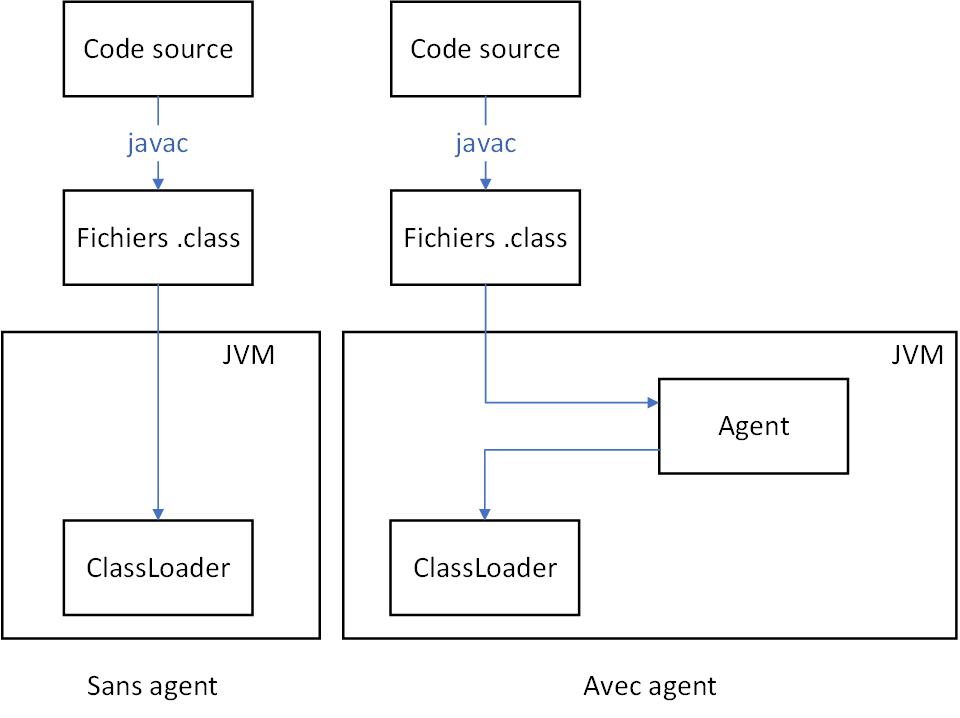
\includegraphics[width=.7\linewidth]{cojac/principle.png}
    \captionof{figure}{Chargement d'une classe}
    \label{fig:cojac_classloading}
\end{minipage}

Cette fonctionnalité est particulièrement utile pour des programmes pouvant fonctionner avec beaucoup d'autres applications. Ils peuvent offrir, par exemple, du monitoring, du profilage, etc.

La majorité des informations dans cette section provient d'une conférence de Rafael Winterhalter \cite{youtube-guide-java-agent}. La première moitié de la conférence se focalise sur la base des \glspl{Java-agent} et des problèmes qui y sont liés. Alors que la seconde moitié se focalise sur Byte Buddy \cite{byte-buddy}, une librairie pour simplifier la transformation de classes.

Il existe deux types d'agents qui seront appelés, dans ce document, agent statique et agent dynamique.

\subsection{Agent statique}

Un agent statique est un \gls{Java-agent} qui est spécifié au démarrage du programme comme c'est le cas avec \gls{COJAC}. Ainsi, lors du démarrage de l'application, l'agent et la \gls{JVM} interagissent ensemble conformément à la Figure \ref{fig:cojac_static_agent}. Cette interaction se déroule en plusieurs étapes:

\begin{enumerate}
    \item La \gls{JVM} appelle l'\gls{Java-agent} en lui donnant le paramètre spécifié (un string) lors du démarrage de l'application. La méthode appelée s'appelle \textit{premain} parce qu'elle est exécutée avant le \textit{main} de l'application cible.
    \item Dans cette méthode \textit{premain}, l'agent doit créer un \textit{ClassFileTransformer}. Cet objet sera utilisé plus tard pour modifié les classes. Cet objet est ensuite donné à la \gls{JVM} grâce à la méthode \textit{Instrumentation.addTransformer}.
    \item Ensuite à chaque fois que la \gls{JVM} veut charger une nouvelle classe, le \textit{ClassLoader} lira le fichier \textit{.class} correspondant.
    \item Le \textit{ClassLoader} enverra ensuite le tableau d'octets qu'il vient de lire au \textit{ClassFileTransformer} qui pourra y apporter les modifications désirées.
    \item Une fois que le \textit{ClassFileTransformer} a modifié la classe, il la retournera la classe à la \gls{JVM}.
\end{enumerate}

\begin{minipage}{\linewidth}% to keep image and caption on one page
\makebox[\linewidth]{%        to center the image
    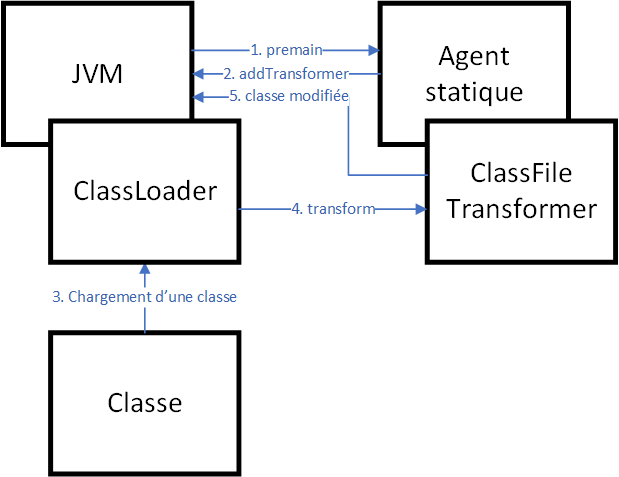
\includegraphics[width=.7\linewidth]{cojac/static_agent.png}
}
\captionof{figure}{Fonctionnement d'un agent statique}
\label{fig:cojac_static_agent}
\end{minipage}

\subsection{Agent dynamique}

Un agent dynamique est un \gls{Java-agent} qui est ajouté après le démarrage de l'application cible. Ceci rend la modification du programme plus complexe et nécessite une autre application pour insérer l'agent. L'ajout de l'agent se déroule en plusieurs étapes comme montré sur la Figure \ref{fig:cojac_dynamic_agent}:

\begin{enumerate}
    \item Une application pour ajouter l'agent doit être créée. Cette application doit s'attacher à la \gls{JVM} du processus dans lequel l'agent doit être inséré. Cette opération ne peut se faire que si l'application cible et l'application source sont sur des processus possédés par le même utilisateur pour des raisons de sécurité.
    \item L'application source charge ensuite l'\gls{Java-agent} dans l'application cible.
    \item Contrairement à l'agent statique, la \gls{JVM} appelle une autre méthode nommée \textit{agentmain}.
    \item L'agent enregistre ensuite son \textit{ClassFileTransformer}.
    \item Cette étape est facultative. Cependant, comme l'application cible a démarrée avant l'agent, elle a déjà chargée certaines classes. La méthode \textit{Instrumentation.\hspace{0pt}retransformClasses} permet de transformer les classes déjà chargées. Cependant, il y a quelques restrictions qui sont listées dans la documentation officielle de cette méthode \cite{java-instrumentation-retransform-documentation}. Pour chaque classe à retransformer, les étapes 6 à 9 seront à nouveau exécutées.
    \item Ensuite à chaque fois que la \gls{JVM} veut charger une nouvelle classe, le \textit{ClassLoader} lira le fichier \textit{.class} correspondant.
    \item Le \textit{ClassLoader} enverra ensuite le tableau de bytes qu'il vient de lire au \textit{ClassFileTransformer} qui pourra y apporter les modifications désirées.
    \item Une fois que le \textit{ClassFileTransformer} a modifié la classe, il la retournera la classe à la \gls{JVM}.
\end{enumerate}

\begin{minipage}{\linewidth}
\makebox[\linewidth]{
    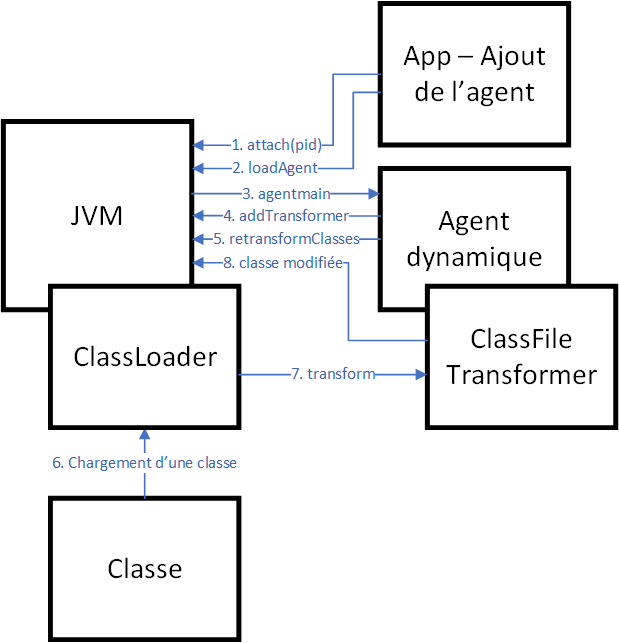
\includegraphics[width=.7\linewidth]{cojac/dynamic_agent.png}
}
\captionof{figure}{Fonctionnement d'un agent dynamique}
\label{fig:cojac_dynamic_agent}
\end{minipage}

\subsection{Synthèse}

Un \gls{Java-agent} permet de modifier le comportement de l'application cible sans en modifier le code source. Cette fonctionnalité permet de faire du profilage, de surveiller des applications ou de modifier le comportement d'une libraire propriétaire.

Les agents statiques et dynamiques ont des objectifs différents. Voici leurs avantages et inconvénients respectifs.

Les agents statiques possèdent les caractéristiques suivantes :

\begin{itemize}
    \item Le changement de l'agent statique nécessite de redémarrer l'application cible.
\end{itemize}

Les agents dynamiques possèdent les caractéristiques suivantes :

\begin{itemize}
    \item La retransformation de classes a d'importantes limitations. Celles-ci sont définies dans la documentation officielle de la méthode correspondante \cite{java-instrumentation-retransform-documentation}.
    \item L'agent peut être ajouté après que l'application ait démarré. Cette fonctionnalité permet, par exemple, de pouvoir obtenir des informations sur une application ayant un bug rare, inconnu ou qui se produit après un certain temps d'activité.
\end{itemize}


\section{Bytecode Java}
\label{sec:bytecode}

Tel que brièvement mentionné dans la section \ref{sec:agent_java} précédente sur les \glspl{Java-agent}, la \textbf{machine virtuelle Java} (\textbf{Java Virtual Machine} ou \textbf{\gls{JVM}}) utilise un seul langage: le \gls{Bytecode} Java. Bien qu'il soit possible de programmer en Java, en Kotlin ou encore en C pour nommer quelques exemples, la \gls{JVM} n'utilise que du \gls{Bytecode}.

Le nom de \gls{Bytecode} provient du fait que chaque code d'opération fait exactement 1 byte. Ceci limite fortement le nombre de codes d'opération disponibles à 256. Certains codes d'opérations peuvent être suivis de paramètres précisant l'opération à effectuer. Voici deux exemples de \gls{Bytecode} dont leur fonctionnement sera illustré plus loin. La première opération prend un byte en paramètre alors que la deuxième opération n'en prend pas.
\begin{minted}{text}
bipush 5
iadd
\end{minted}

Contrairement aux processeurs habituels, la \gls{JVM} utilise une pile au lieu de registres. Certaines opérations permettent de charger des informations sur la pile ou d'y retirer un élément pour le stocker dans une variable. Toutes les autres opérations prennent comme entrée les valeurs sur la pile et ajoutent le résultat sur cette même pile.

Voici un exemple de \gls{Bytecode} qui permet de mettre deux integers sur la pile et de les additionner:
\begin{minted}{text}
bipush 5
bipush 7
iadd
\end{minted}

\begin{minipage2}
L'exécution de ce \gls{Bytecode} est illustrée sur la Figure \ref{fig:cojac_bytecode_stack_addition}. Pour cet exemple, la pile est vide avant d'exécuter ces commandes. L'exécution se déroule en plusieurs étapes:

\begin{enumerate}
    \item Le nombre 5 est ajouté sur la pile.
    \item Le nombre 7 est ajouté sur la pile.
    \item L'addition consomme les deux nombres et ajoute le résultat sur la pile.
\end{enumerate}
\end{minipage2}

\begin{minipage}{\linewidth}% to keep image and caption on one page
\makebox[\linewidth]{%        to center the image
    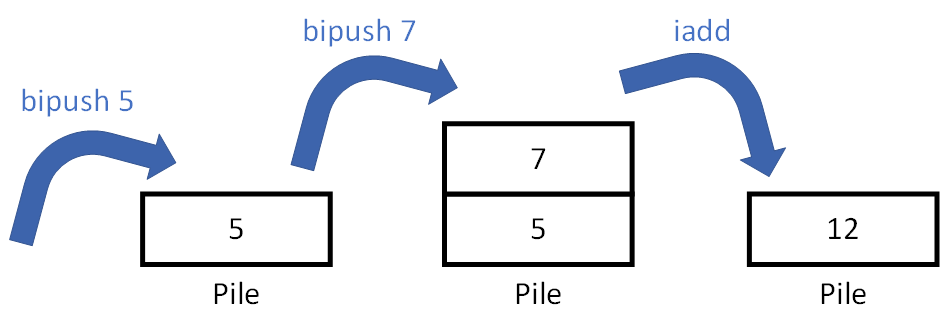
\includegraphics[width=.7\linewidth]{cojac/stack_addition_example.png}
}
\captionof{figure}{Addition de deux nombres en Bytecode Java}
\label{fig:cojac_bytecode_stack_addition}
\end{minipage}

Des informations plus complètes sont disponibles dans une conférence intitulée "Java Bytecode Crash Course" de David Buck, un ingénieur chez Oracle \cite{java-bytecode-video}.

Les spécifications de chaque instruction sont aussi définies dans la documentation officielle d'Oracle \cite{java-bytecode-documentation}.

\section{Intégration}
\label{sec:cojac_integration}

\gls{COJAC} propose deux manières d'intégrer une nouvelle fonctionnalité:

\begin{itemize}
    \item \textbf{\Gls{Behaviour}}: les opérations sur les floats et les doubles sont simplement remplacées par un appel de méthode. Ainsi, il est possible de changer le comportement de ceux-ci. Dans ce projet, il serait possible de mettre la partie réelle et la partie imaginaire dans un double et de modifier les opérations qui les utilisent.
    \item \textbf{Wrapper}: les floats et les doubles peuvent être remplacés par un objet (wrapper). Ce qui permet d'ajouter plus d'éléments dans le wrapper.
\end{itemize}

Le \gls{Behaviour} a les caractéristiques suivantes:

\begin{itemize}
    \item Le stockage est limité en taille (8 octets pour un double).
    \item Moins de modifications sont nécessaires. Toutes les opérations sur les doubles et les appels de la méthodes de la librairie standard doivent être modifiés. Il est également possible de convertir les floats en doubles. A ce moment, il y a beaucoup plus de modifications.
\end{itemize}

Le \gls{Wrapper} a les caractéristiques suivantes:

\begin{itemize}
    \item Le stockage est illimité.
    \item Beaucoup de modifications doivent être effectuées. Toutes les constantes, signatures de méthode, opérations, etc. doivent être adaptées parce qu'un type de base et un objet sont radicalement différents.
\end{itemize}

\subsection{Ajout d'un wrapper}

Pour ajouter un nouveau \gls{Wrapper} dans \gls{COJAC}, il faut créer une nouvelle classe dans le package \textit{com.github.cojac.models.wrappers}. Cette nouvelle classe doit hériter de la classe abstraite \textit{ACojacWrapper}. Il faut ensuite implémenter toutes les méthodes.

On peut ensuite tester le nouveau \gls{Wrapper} en suivant ces deux étapes:

\begin{enumerate}
    \item Créer le \gls{JAR} de \gls{COJAC}
    \item Démarrer l'application cible en donnant le \gls{JAR} créé précédemment comme \gls{Java-agent} et lui donner le \gls{Wrapper} à utiliser avec l'option \textit{-W}. Pour démarrer une application avec un \gls{Wrapper} nommé \textit{WrapperComplexNumber}, la commande suivante sera utilisée:
    \begin{minted}[breaklines]{shell}
java -javaagent:cojac.jar="-W cojac.WrapperComplexNumber" demo.HelloComplexNumber
    \end{minted}
\end{enumerate}

\subsection{Limitations}

La documentation de COJAC \cite{cojac-wiki-limitations} prévient que les \glspl{Wrapper} de \gls{COJAC} sont encore expérimentaux et qu'ils possèdent les limitations suivantes:

\begin{itemize}
    \item Il y a des problèmes dans les transitions entre le code utilisateur et la librairie standard Java. Par exemple, lors de l'utilisation de tableaux de nombres.
    \item Les "callbacks" de la bibliothèque Java vers le code utilisateur lorsque des nombres à virgule flottante sont transmis ne sont pas supportés.
    \item L'instruction \gls{Bytecode} \textit{invokedynamic} devrait fonctionner pour Java 8, mais cela n'est pas garanti. De plus, les nouvelles utilisations de cette instruction tel que mentionné dans la section \ref{sec:problem_cojac_instrumentation} ne sont pas supportés.
    \item L'utilisation de la \textit{Java reflection} n'est pas supportée.
    \item La conversion des types primitifs (float/double) et de leur \gls{Wrapper} original (Float/\hspace{0pt}Double) provoquent certains problèmes tels que des conflits de signatures de méthodes ou des erreurs de comparaison.
    \item L'implémentation des modèles n'est pas optimale. Par exemple, les appels à la librairie standard \textit{Math.*} ne calculent pas les valeurs aussi précisément que demandées.
    \item Il y a également un ralentissement important.
\end{itemize}

\subsection{Méthodes magiques}

\Gls{COJAC} offre aussi un mécanisme de méthodes magiques. Ces méthodes permettent à l'application cible d'utiliser du code de \gls{COJAC}. Le principe qui se cache derrière se mécanisme est bien documenté dans la section 5.4 d'un rapport précédent sur les nombres enrichis dans COJAC \cite{enriched-numbers}.

\section{Maven}

\gls{COJAC} utilise \gls{Maven} \cite{maven} pour créer le \gls{JAR}. \gls{Maven} est un outil d'automatisation pour gérer les dépendances et produire une application. Cet outil peut télécharger les dépendances, compiler le projet, exécuter les tests unitaires et d'intégration et déployer le projet. \gls{Maven} et Gradle sont les deux outils les plus souvent utilisés pour gérer les projets Java. Toute la configuration se trouve dans le fichier \textit{pom.xml}.

\subtitle{Debug}
\label{sec:cojac_maven_debug}

Lorsqu'il y a un problème avec \gls{Maven}, il y a plusieurs paramètres qui permettent d'obtenir plus d'informations. Cette section montre comment configurer ces paramètres sous IntelliJ et donne l'argument équivalent pour appeler \gls{Maven} en ligne de commande.

\begin{minipage2}
\subtitle{Ouvrir la fenêtre Maven}

Toutes les configurations effectuées ci-dessous seront effectuées depuis la fenêtre \gls{Maven} dans IntelliJ. Le bouton pour l'ouvrir se situe sous \textbf{View} $\rightarrow$ \textbf{Tool Windows} $\rightarrow$ \textbf{Maven} comme montré sur la Figure \ref{fig:maven_open_window}.
\end{minipage2}

\begin{minipage}{\linewidth}% to keep image and caption on one page
\makebox[\linewidth]{%        to center the image
    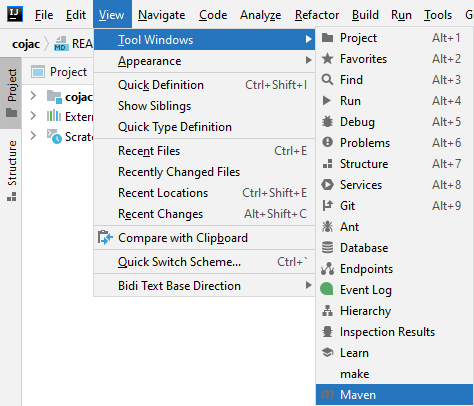
\includegraphics[width=.7\linewidth]{maven/open_maven_window.png}
}
\captionof{figure}{Bouton d'ouverture de la fenêtre \gls{Maven}}
\label{fig:maven_open_window}
\end{minipage}

\subtitle{Fenêtre Maven}

La fenêtre \gls{Maven} montre le contenu du projet avec les étapes du cycle de vie de la production de l'application comme le montre la Figure \ref{fig:maven_window}. Le bouton encadré sur l'image permet d'ouvrir les paramètres de \gls{Maven} qui seront utilisés plus tard. On peut également voir les plugins et les dépendances. Cette fenêtre permet aussi d'exécuter les étapes pour produire l'application. L'étape \textit{package} est suffisante pour générer le \gls{JAR}.

\begin{minipage}{\linewidth}
\makebox[\linewidth]{
    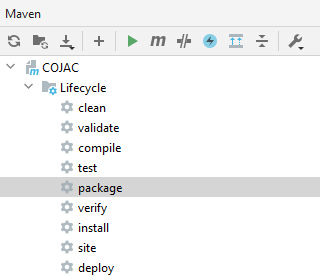
\includegraphics[width=.5\linewidth]{maven/maven_window_annotated.png}
}
\captionof{figure}{Fenêtre \gls{Maven}}
\label{fig:maven_window}
\end{minipage}

Une option peut être ajoutée pour afficher les messages de debug. Cette option est plus souvent utilisée lors du développement de \gls{Maven} ou d'un plugin \gls{Maven}. Cependant, elle peut également être utile pour trouver la source d'un problème difficile. Cette option est visible sur la Figure \ref{fig:maven_debug}. L'option en ligne de commande équivalente se nomme \textit{-{}-debug}.

\begin{minipage}{\linewidth}
\makebox[\linewidth]{
    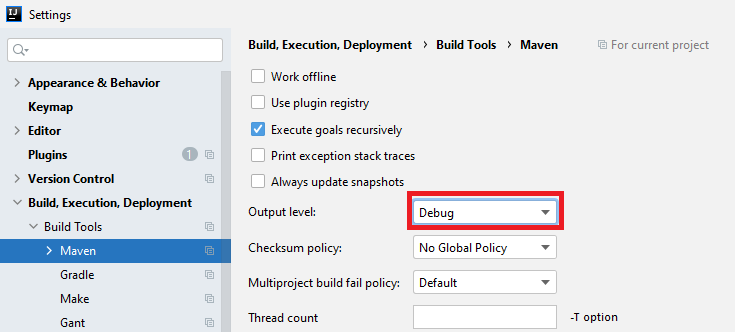
\includegraphics[width=\linewidth]{maven/maven_debug.png}
}
\captionof{figure}{Configuration d'affichage des messages de debug}
\label{fig:maven_debug}
\end{minipage}

\chapter{Intégration des nombres complexes}

\section{Nombres complexes}

Lorsque l'humanité à créer les nombres, ils étaient limités aux entiers positifs. L'humanité y a progressivement inclus des nombres négatifs, puis des nombres réels. Cependant, bien que ces nombres suffisent en général, d'autres ensemble de nombres plus larges existent également comme les nombres complexes qui sont le sujet de ce chapitre.

\subsection{Avantages}

Bien que ces nombres complexes étaient considérés comme une astuce pour résoudre des problèmes ayant des racines carrés de nombres négatifs, ces nombres sont désormais très souvent utilisés en mathématique, en physique et en ingénierie. Ils permettent de simplifier l'écriture de nombreuses formules et sont suffisants pour décrire une grande majorité des lois et phénomènes physiques.

Une raison majeure de la nécessité d'intégrer dans l'arsenal mathématique le corps des nombres complexes tient au fait qu'il est algébriquement clos. C'est-à-dire que chaque polynôme complexe de degré 1 ou supérieur a au moins une racine complexe. Ainsi, il n'y a pas les mêmes risques que pour les nombres réels où chaque calcul de racine doit être fait avec précautions sans quoi, il pourrait n'exister aucune solution dans le domaine réel. Avec les nombres complexes, il est garanti qu'une racine existera nécessairement.

Les nombres complexes ont eux aussi des limites, même si on ne les rencontre que rarement. C'est seulement dans des cas spécifiques, tel que la physique quantique avec un spin, que les nombres complexes se révèlent insuffisants.

\subsection{Désavantages}

Les nombres complexes ont aussi un désavantage: la perte de comparaison. Comme les nombres réels peuvent être représentés sur un axe, il est toujours possible de définir si un nombre est plus petit ou plus grand qu'un autre. Cette même comparaison n'a plus lieu d'être avec les nombres complexes, car il ne s'agit plus d'un axe, mais d'un espace à 2 dimensions. Selon les situations, les nombres complexes peuvent être comparés par leur partie réelle, par leur partie imaginaire, par leur module ("la taille" de ce nombre), etc.

\subsection{Représentations}
\label{sec:complex_representations}

Les nombres complexes peuvent être écrits sous différentes formes:
\begin{itemize}
    \item Algébrique: $a + bi$ où $a$ est la partie réelle et $bi$ est la partie imaginaire. Ex: $3 - 2i$
    \item Trigonométrique: $r(cos(\theta) + i \cdot sin(\theta))$
    \item Exponentielle: $re^{i\theta}$
    \item Polaire: $(r, \theta)$
\end{itemize}

Voici l'exemple du nombre $3 - 2i$ visible sur la figure \ref{fig:complex_3-2i}.

\begin{minipage}{\linewidth}
\makebox[\linewidth]{
    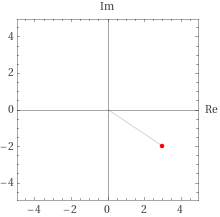
\includegraphics[width=.5\linewidth]{complex_numbers/3-2i.png}
}
\captionof{figure}{Le nombre $3 - 2i$ dans l'espace complexe}
\label{fig:complex_3-2i}
\end{minipage}

Voici les différentes notations correspondant toutes au nombre $3 - 2i$:
\begin{itemize}
    \item Algébrique: $3 - 2i$
    \item Trigonométrique: $\sqrt{13} \cdot (cos(-tan^{-1}(\frac{2}{3})) + i \cdot sin(-tan^{-1}(\frac{2}{3})))$
    \item Exponentielle: $\sqrt{13} \cdot e^{-i \cdot tan^{-1}(\frac{2}{3})}$
    \item Polaire: $(\sqrt{13}, -tan^{-1}(\frac{2}{3}))$
\end{itemize}

Dans chaque de ces formes, on connaît soit la partie réelle et la partie imaginaire, soit l'angle et le module (ou rayon) du nombre complexe. On peut passer de l'un à l'autre en utilisant les formules de Pythagore et de trigonométrie. \todo{Ajouter formules}


\section{Spécifications}

Les calculs seront réalisé avec les \glspl{Unums} autant que possible. Les \textit{floats} et les \textit{doubles} auront le même comportement pour les autres méthodes (\textit{toString}, \textit{parseDouble}, etc.). Les \glspl{Unums} doivent fonctionner au moins sur une plateforme. Si seulement quelques plateformes sont supportés, il est nécessaire de décrire la procédure pour porter cette fonctionnalité sur une nouvelle plateforme.

\section{Démonstration}

La démonstration se base sur deux exemples donnés par M. John L. Gustafson.

En utilisant les formules suivantes: $E(0) = 1, E(z) = \frac{e^z - 1}{z}, Q(x) = |x - \sqrt{x^2 + 1}| - \frac{1}{x+\sqrt{x^2 + 1}}$, la fonction suivante $H(x) = E(Q(x)^2)$ évaluée avec les valeurs 15, 16, 17 et 9999 doit valoir 1.

Lorsque ce calcul est réalisé en \textit{double precision}, le résultat est toujours 0. Le code utilisé est le suivant:

\begin{minted}{Java}
private static double func1E(double a) {
    if (a == 0) return 1;
    return (Math.exp(a) - 1) / a;
}

private static double func1Q(double a) {
    double sqrt = Math.sqrt(a * a + 1);
    return Math.abs(a - sqrt) - 1 / (a + sqrt);
}

public static double func1H(double a) {
    double q = func1Q(a);
    return func1E(q * q);
}

public static void main(String[] args) {
    // example from https://youtu.be/jN9L7TpMxeA?t=1994
    double[] inputs = new double[]{15, 16, 17, 9999};
    for (double input : inputs) {
        double result = func1H(input);
        System.out.println(result + " should be 1.0");
    }
}
\end{minted}

Le deuxième exemple est un produit scalaire de 2 vecteurs particuliers. Lors des tests, le \textit{double precision} est suffisant pour obtenir le bon résultat contrairement aux résultats obtenus par M. John L. Gustafson. Ceci peut s'expliquer par le fait que les calculs ne sont pas forcément identiques entre des machines différentes et que la norme IEEE-754 \cite{ieee-754-2019} a de nombreuses options facultatives.

\begin{minipage2}
Le produit scalaire est implémenté de la manière suivante:

\begin{minted}{Java}
public static float scalarProduct(float[] a, float[] b) {
    assert (a.length == b.length);
    float result = 0f;
    for (int i = 0; i < a.length; i++) {
        result = Math.fma(a[i], b[i], result);
    }
    return result;
}

public static void main(String[] args) {
    // example from https://youtu.be/aP0Y1uAA-2Y?t=104
    float[] a = new float[]{3.2e7f, 1, -1, 8.0e7f};
    float[] b = new float[]{4.0e7f, 1, -1, -1.6e7f};
    float result = scalarProduct(a, b);
    System.out.println(result + " should be 2.0");
}
\end{minted}
\end{minipage2}

La longueur minimale pour que ces exemples fonctionnent n'est pas connue.

\chapter{Conception}

Ce chapitre contient la conception de l'intégration des nombres complexes dans COJAC \cite{COJAC}.

\section{Approche}
\label{sec:complex_approach}

Comme expliqué dans la section \ref{sec:cojac_integration}, l'intégration des nombres complexes peut se faire à l'aide de deux mécanismes différents:
\begin{itemize}
    \item Behaviour: réinterprétation des \textit{floats} et des \textit{doubles}.
    \item Wrapper: remplacement des \textit{floats} et des \textit{doubles} par un wrapper.
\end{itemize}

L'intégration des nombres complexes se fera en utilisant un wrapper afin de pouvoir garder la \textit{double precision}.

\section{Comparaison}

La comparaison entre les nombres complexes est un problème important. Toutes les comparaisons entre les nombres sont faites à l'aide d'une même opération et il faut aussi que les comparaisons entre des nombres purement réels soient respectés. Ainsi si on compare des nombres complexes (avec une partie imaginaire), il n'y a pas forcément de valeurs de retour adaptées car il n'y a pas d'ordre total avec les nombres complexes. Cette situation peut être montrée avec l'exemple de code suivant:

\begin{minted}{Java}
double a = ...;
if (a == 0) {
    System.out.println("a = 0");
} else {
    System.out.println("a != 0");
}
\end{minted}

Si la variable \textit{a} est purement réel, ce code doit fonctionner. Cependant il y a un problème si la variable \textit{a} est complexe. Pour cet exemple, la valeur de \textit{a} sera \textit{2i}. Lorsque le remplacement de cet opération est faite, la méthode doit comparer ces deux nombres (\textit{2i} et 0) et retourner une valeur parmi les trois suivantes:

\begin{itemize}
    \item \textit{2i} < 0
    \item \textit{2i} = 0
    \item \textit{2i} > 0
\end{itemize}

Cependant, aucune de ces réponses n'est vraie. Il est possible de créer une méthode magique pour gérer les égalités, mais ceci nécessitera que l'application cible soit modifiée pour réaliser la comparaison.

Comme aucun des deux choix n'est complètement satisfaisant, une option supplémentaire pour COJAC \cite{COJAC} sera disponible pour choisir le comportement des comparaisons.



\begin{tabularx}{\columnwidth}{| p{6em} | X | X |}
    \hline
     & \textbf{Sans option: pas d'erreur} & \textbf{Avec option: erreur et méthodes magiques} \\
    \hline
    Principe:
    & La comparaison se fera d'abord avec la partie réelle, puis avec la partie complexe. Ainsi \textit{2 - i} sera considéré comme plus petit que \textit{2}.
    & La comparaison sera mathématiquement correcte. La comparaison entre deux nombres purement réels donnera toujours un résultat. La comparaison entre deux nombres complexes égaux donnera également un résultat correct. Dans les autres cas, une exception sera générée. \\
    & & Une méthode magique permettra de vérifier l'égalité de deux nombres complexes. Elle retournera un booléen même en cas d'inégalité. Deux méthodes magiques permettant de garder que la partie réelle ou imaginaire d'un nombre complexe sera aussi disponible et permettra à l'utilisateur d'implémenter lui-même la comparaison entre les nombres complexes.\\
    \hline
    Avantage:
    & Ceci permet de fonctionner sans modifier le code de l'application cible. Ceci respecte au maximum l'ordre établi entre les nombres réels.
    & La comparaison est mathématiquement correcte. Ainsi, l'utilisateur est conscient des problèmes qui peuvent se produire lorsqu'il travaille avec les nombres complexes. \\
    & & L'usage des méthodes magiques permet une plus grande flexibilité avec les nombres magiques. \\
    \hline
    Désavantage:
    & Un ordre total est défini alors qu'il n'existe pas mathématiquement. Ceci peut conduire à des comparaisons donnant un résultat mathématiquement faux et produire des incohérences.
    & L'application cible doit être écrite en tenant compte des fonctions magiques de COJAC \cite{COJAC}. \\
    \hline
\end{tabularx}

\begin{minipage2}
Voici un exemple d'incohérence pouvant apparaître avec la première solution (pas d'erreur, ordre absolu).

\begin{minted}{Java}
double[] sorted_positives = ... // ex: new double[]{2 + 3i, 3, 1};
Arrays.sort(sorted_positives); // sorted_positives = [1, 2 + 3i, 3]
double[] sorted_abs = new double[sorted_positives.length];
for (int i = 0; i < sorted_positives.length; i++){
    sorted_abs[i] = Math.abs(sorted_positives[i]);
}
// sorted_abs = [1, 3.6, 3]
\end{minted}
\end{minipage2}

Si ce code est exécuté avec des nombres réels, le tableau \textit{sorted\_abs sera trié}. Lorsque ce même code est exécuté avec des nombres complexes, le tableau \textit{sorted\_abs sera trié} ne sera pas trié dû à la définition de la valeur absolue d'un nombre complexe.

\section{Diagramme de classes}

Toutes les méthodes abstraites du \textit{ACojacWrapper} seront implémentées en plus de la méthode \textit{isNaN}. De plus, une nouvelle méthode sera ajoutée sur \textit{ACojacWrapper} afin de pouvoir supporter la méthode \textit{Math.cbrt}.

\todo{ajouter diagramme}

\section{Librairie disponible}

La librairie \textit{commons-math3} est déjà disponible en Java pour gérer les nombres complexes \cite{apache-complex-documentation}. Elle possède beaucoup de fonctionnalités et implémente déjà la grande majorité des opérations mathématiques nécessaires. De plus, cette librairie fait déjà partie des dépendances de ce projet.

\section{Implémentation}

\subsection{Wrapper}

La création d'un nouveau wrapper se fait en créant une nouvelle classe héritant de \textit{ACojacWrapper}. Comme \textit{ACojacWrapper} est une classe abstraite, le wrapper ne peut pas étendre d'autres classes.

Il faut également implémenter un constructeur prenant un \textit{ACojacWrapper} en paramètre. Il faut également gérer le cas où ce paramètre est null. Voici le constructeur implémenté pour ce wrapper:

\begin{minted}{Java}
public WrapperComplexNumber(ACojacWrapper w) {
    // CommonDouble can call this constructor with a null wrapper
    if (w == null) {
        this.complex = new Complex(0, 0);
    } else {
        Complex value = ((WrapperComplexNumber) w).complex;
        this.complex = new Complex(value.getReal(), value.getImaginary());
    }
}
\end{minted}

\subsection{Remplacement de méthodes}

Seulement une sélection de méthodes de la librairie standard sont remplacées. Deux méthodes supplémentaires sont également remplacées car elles sont utilisées dans la démonstration. Il s'agit de:
\begin{itemize}
    \item \textit{Math.cbrt(double)}
    \item \textit{Double.isNaN(double)}
\end{itemize}

Le remplacement des méthodes de la librairie standard pour les wrappers se fait dans la classe \textit{com.github.cojac.instrumenters.ReplaceFloatsMethods} dans la méthode \textit{fillMethods}. Les lignes suivantes ont été ajoutées pour remplacer ces deux méthodes supplémentaires:

\begin{minted}[breaklines]{Java}
// String CDW; // signature of wrapper
// String CDW_N; // name of wrapper
invocations.put(new MethodSignature(DL_NAME, "isNaN", "(D)Z"),
new InvokableMethod(CDW_N, "double_isNaN", "(" + CDW + ")Z", INVOKESTATIC));

invocations.put(new MethodSignature(MATH_NAME, "cbrt", "(D)D"),
new InvokableMethod(CDW_N, "math_cbrt", "(" + CDW + ")" + CDW, INVOKESTATIC));
\end{minted}

Il faut également ajouter les deux méthodes déclarées ici: \textit{double\_isNaN} and \textit{math\_cbrt} dans la classe \textit{com.github.cojac.models.wrappers.CommonDouble} et les faire appeler la méthode correspondante du wrapper:

\begin{minted}{Java}
public static boolean double_isNaN(CommonDouble a){
    return a.val.isNaN();
}

public static CommonDouble math_cbrt(CommonDouble a){
    return new CommonDouble(a.val.math_cbrt());
}
\end{minted}

\subsection{Ajout de l'option}

Une nouvelle option doit aussi être ajoutée à COJAC pour que le wrapper puisse être utilisé et configuré. Tout d'abord, il faut ajouter une valeur dans l'enum \textit{com.github.cojac.Arg}.

\begin{minted}{Java}
COMPLEX_NUMBER ("Rc"),
\end{minted}

Cette enum a aussi une méthode \textit{createOptions}. Il faut aussi y ajouter une option. Ceci permettra de rendre l'option publique et utilisable comme argument et permettra aussi d'afficher l'aide à propos de cette option. Voici le code pour ajouter une option avec un argument facultatif:

\begin{minted}[breaklines]{Java}
options.addOption(OptionBuilder
    .withArgName("strict")
    .hasOptionalArg()
    .withDescription("Use complex number wrapping. Strict mode generates an exception when the imaginary " +
            "part is lost or when a comparison between two different complex numbers is made.")
    .create(COMPLEX_NUMBER.shortOpt()));
\end{minted}

Il faut aussi détecter quand l'option est utilisée et la traiter en conséquence. Pour ce faire, il faut ajouter une condition dans la classe \textit{com.github.cojac.CojacReferences.CojacReferencesBuilder} à l'intérieur de la méthode \textit{build}. Ce code doit être ajouté suffisamment haut dans la méthode car elle définit l'option \textit{Arg.NG\_WRAPPER} qui est aussi traitée dans la même méthode. Voici l'extrait de code qui permet de traiter cette option:

\begin{minted}[breaklines]{Java}
if (args.isSpecified(Arg.COMPLEX_NUMBER)) {
    args.setValue(Arg.NG_WRAPPER, "com.github.cojac.models.wrappers.WrapperComplexNumber");
    WrapperComplexNumber.setStrictMode( args.getValue(Arg.COMPLEX_NUMBER) != null);
}
\end{minted}

\subsection{\textit{toString} et \textit{fromString}}

La méthode \textit{toString} a été implémentée pour avoir trois formats possibles d'après le type de nombres complexes.

\begin{itemize}
    \item Nombre réel: uniquement la partie réelle (ex: 2.25).
    \item Nombre imaginaire: uniquement la partie réelle avec un \textit{i} à la fin (ex: -4.2i).
    \item Nombre complexe: les deux parties sont affichées (ex: -4.25 + 4.0i ou 1.25 - 1.5i).
\end{itemize}

Ces deux méthodes se basent sur l'affichage du double de Java. Ainsi, \textit{1.401298464324817E-45 - 1.0i} est une représentation possible d'un nombre complexe et il est aussi possible de convertir cette chaîne de caractères en un nombre complexe.

La méthode \textit{fromString} est capable de lire et de créer un nombre complexe à partir de tous les exemples de String valides donnés précédemment.

Cependant, des modifications ont dû être effectuées parce que les méthodes \textit{Float.parseFloat} et \textit{Double.parseDouble} appellent les méthodes des classes \textit{CommonFloat} et \textit{CommonDouble}. Cependant, ces classes font ensuite elles-même un appel aux vraies méthodes \textit{Float.parseFloat} et \textit{Double.parseDouble}.

Voici l'ancien code du \textit{CommonDouble}:

\begin{minted}{Java}
public CommonDouble(String v) {
    this(Double.valueOf(v));
}

public static CommonDouble fromString(String a){
    return fromDouble(Double.valueOf(a));
}
\end{minted}

\begin{minipage2}
Et voici le nouveau code qui fait l'appel à une nouvelle méthode du \textit{ACojacWrapper}:

\begin{minted}{Java}
public CommonDouble(String v) {
    val = newInstance(null).fromString(v, false);
}

public static CommonDouble fromString(String a){
    return new CommonDouble(a);
}
\end{minted}
\end{minipage2}


\section{Tests}

Cette section décrit l'ensemble des tests unitaires et d'intégration réalisés pour vérifier le fonctionnement du wrapper. Tous les tests écrits se déroulent avec succès.

\subsection{Tests unitaires}

Toutes les méthodes ont été testées avec au moins un cas général. Les cas particuliers n'ont pas été testés. Ceci inclus les grands nombres, les nombres tout petits et autres valeurs spéciales (NaN, null, etc.). Quelques tests plus précis ont été ajoutés pour éviter que certains bugs, qui ont été corrigés depuis, se reproduisent.

55 tests unitaires ont été réalisés. De plus, ces tests couvrent 100\% de la classe \textit{WrapperComplexNumber}. Les détails sont visibles dans le tableau suivant:

\begin{table}[h]
    \begin{tabularx}{\columnwidth}{ | p{12em} | X | X | X |}
        \hline
        \textbf{Élément} & \textbf{Classe} & \textbf{Méthodes} & \textbf{Lignes} \\
        \hline
        WrapperComplexNumber & 100\% (1/1) & 100\% (47/47) & 100\% (118/118) \\
        \hline
    \end{tabularx}
\end{table}

\subsection{Tests d'intégration}

Des tests d'intégrations ont aussi été réalisés. Une classe de test est instrumentée et le retour de ces méthodes sont vérifiées. 13 tests ont été réalisés en mode normal et 14 tests en mode strict.


\section{Documentation}

Quelques commentaires ont été ajoutés dans le code à quelques endroits spécifiques pour expliquer les choix réalisés. Comme les tests d'intégration sont séparés en deux classes, le retour attendu a aussi été documenté car la vérification des valeurs se fait uniquement dans la deuxième classe. Aucun autre commentaire n'a été ajouté parce qu'ils n'apportaient que peu de valeur parce que les méthodes sont généralement courtes et explicites.

Une nouvelle section dans le wiki décrit désormais aussi le \gls{Wrapper} des \glspl{Complex-number}. Cette section détaille également les deux modes disponibles et montre également un code de démonstration.

\section{Résultats}

L'implémentation des \glspl{Complex-number} fonctionnent correctement. Des tests unitaires et d'intégration assurent également la fiabilité de cette implémentation. La démonstration donne également le résultat attendu et montre l'intérêt de cette fonctionnalité. Cette fonctionnalité est aussi documentée dans le wiki.

% ==============
% Description of all problems that happened during the project
% ==============

\chapter{Problèmes rencontrés}

\section{Surefire provoque une exception lors de l'exécution des tests par Maven}

Surefire provoquait une erreur lors de l'exécution des tests lorsqu'un espace était présent dans le chemin d'accès.

\subsection{Problème}
\label{sec:problems_surefire_problem}

Lors de la création du JAR, l'erreur suivante se produit lors de l'exécution des tests:

\begin{minted}[breaklines]{text}
ExecutionException The forked VM terminated without properly saying goodbye. VM crash or System.exit called?
\end{minted}

Le message suivant présent dans les logs indique la localisation des fichiers qui contiennent plus de détails.
\begin{minted}[breaklines]{text}
[ERROR] Please refer to D:\Documents\Documents\HEIA\Semestre 6 - 2021\Bachelor\Projet\cojac\target\surefire-reports for the individual test results.
\end{minted}

\subsection{Solution temporaire: ne pas exécuter les tests}

Comme les problèmes ont uniquement lieu durant les tests, il est possible de générer le JAR sans les exécuter. \todo{lien section Maven} Pour ce faire, il faut cliquer sur le bouton dédié dans la fenêtre Maven. Ce bouton est visible sur la figure \ref{fig:problems_maven_skip_tests}.

Cependant, cette solution ne doit être utilisée que s'il y a besoin du JAR pour d'autres raisons. Il est nécessaire de corriger ce problème pour garantir la qualité du code.

\begin{minipage}{\linewidth}
\makebox[\linewidth]{
    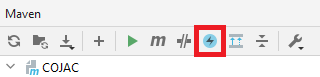
\includegraphics[width=.5\linewidth]{problems/maven_skip_tests.png}
}
\captionof{figure}{Bouton pour ignorer les tests}
\label{fig:problems_maven_skip_tests}
\end{minipage}

\subsection{Cause}

Dans un des fichiers de log produits, qui sont mentionnées dans la section \ref{sec:problems_surefire_problem}, on peut trouver l'erreur suivante:

\begin{minted}[breaklines]{text}
# Created at 2021-06-03T14:09:01.042
Error opening zip file or JAR manifest missing : D:\Documents\Documents\HEIA\Semestre
\end{minted}

Ce lien est incomplet par rapport au chemin mentionné dans la section \ref{sec:problems_surefire_problem}. Le chemin d'accès s'arrête lors du premier espace trouvé. Si le projet est déplacé dans un dossier ne contenant aucun espace, le JAR est correctement généré.

\subsection{Solution}

Il faut modifier une ligne de configuration du plugin Surefire dans le \textit{pom.xml}. Des guillemets ont été ajoutés autour du chemin d'accès du JAR pour obtenir la ligne suivante.
\inputmintedcolor{xml}{code/maven-surefire-javaagent.xml}

Ce changement corrige le problème.

\section{Erreur lors de l'instrumentation d'une application par COJAC}

Lors de l'appel de la commande pour instrumenter une démonstration avec COJAC \cite{COJAC}, COJAC \cite{COJAC} provoque une erreur.

\subsection{Problème}

L'application peut être démarrée sans COJAC \cite{COJAC} avec la commande suivante:
\begin{minted}{bat}
java demo\HelloBigDecimal.java
\end{minted}

Cependant, COJAC \cite{COJAC} produit une erreur lorsque l'application est démarrée avec COJAC \cite{COJAC}. La commande suivante a été utilisée:
\begin{minted}{bat}
java -javaagent:cojac.jar="-Rb 50" demo\HelloBigDecimal.java
\end{minted}

\subsection{Solution temporaire: compiler avec Java 8}

COJAC \cite{COJAC} doit être compilé avec Java 9 au minimum, mais l'application instrumentée doit être compilée avec Java 8. Les deux commandes suivantes permettent de compiler une démonstration et de l'exécuter:
\begin{minted}{bat}
javac -source 8 -target 8 demo\HelloBigDecimal.java
java -javaagent:cojac.jar="-Rb 50" demo.HelloBigDecimal
\end{minted}

\subsection{Cause}

La source du problème provient de l'instruction Bytecode \textit{Invokedynamic} qui a évolué en Java 9 et qui est désormais utilisé pour de nouvelles opérations qui ne sont pas supportés par COJAC \cite{COJAC} à l'heure actuelle.

\printbibliography

\begin{appendices}

\section{Spécifications}

Les calculs seront réalisé avec les \glspl{Unums} autant que possible. Les \textit{floats} et les \textit{doubles} auront le même comportement pour les autres méthodes (\textit{toString}, \textit{parseDouble}, etc.). Les \glspl{Unums} doivent fonctionner au moins sur une plateforme. Si seulement quelques plateformes sont supportés, il est nécessaire de décrire la procédure pour porter cette fonctionnalité sur une nouvelle plateforme.

\section{Démonstration}

La démonstration se base sur deux exemples donnés par M. John L. Gustafson.

En utilisant les formules suivantes: $E(0) = 1, E(z) = \frac{e^z - 1}{z}, Q(x) = |x - \sqrt{x^2 + 1}| - \frac{1}{x+\sqrt{x^2 + 1}}$, la fonction suivante $H(x) = E(Q(x)^2)$ évaluée avec les valeurs 15, 16, 17 et 9999 doit valoir 1.

Lorsque ce calcul est réalisé en \textit{double precision}, le résultat est toujours 0. Le code utilisé est le suivant:

\begin{minted}{Java}
private static double func1E(double a) {
    if (a == 0) return 1;
    return (Math.exp(a) - 1) / a;
}

private static double func1Q(double a) {
    double sqrt = Math.sqrt(a * a + 1);
    return Math.abs(a - sqrt) - 1 / (a + sqrt);
}

public static double func1H(double a) {
    double q = func1Q(a);
    return func1E(q * q);
}

public static void main(String[] args) {
    // example from https://youtu.be/jN9L7TpMxeA?t=1994
    double[] inputs = new double[]{15, 16, 17, 9999};
    for (double input : inputs) {
        double result = func1H(input);
        System.out.println(result + " should be 1.0");
    }
}
\end{minted}

Le deuxième exemple est un produit scalaire de 2 vecteurs particuliers. Lors des tests, le \textit{double precision} est suffisant pour obtenir le bon résultat contrairement aux résultats obtenus par M. John L. Gustafson. Ceci peut s'expliquer par le fait que les calculs ne sont pas forcément identiques entre des machines différentes et que la norme IEEE-754 \cite{ieee-754-2019} a de nombreuses options facultatives.

\begin{minipage2}
Le produit scalaire est implémenté de la manière suivante:

\begin{minted}{Java}
public static float scalarProduct(float[] a, float[] b) {
    assert (a.length == b.length);
    float result = 0f;
    for (int i = 0; i < a.length; i++) {
        result = Math.fma(a[i], b[i], result);
    }
    return result;
}

public static void main(String[] args) {
    // example from https://youtu.be/aP0Y1uAA-2Y?t=104
    float[] a = new float[]{3.2e7f, 1, -1, 8.0e7f};
    float[] b = new float[]{4.0e7f, 1, -1, -1.6e7f};
    float result = scalarProduct(a, b);
    System.out.println(result + " should be 2.0");
}
\end{minted}
\end{minipage2}

La longueur minimale pour que ces exemples fonctionnent n'est pas connue.

\end{appendices}

\printglossaries

\end{document}